\documentclass[border=4pt]{standalone}
\usepackage{tikz}

\begin{document}
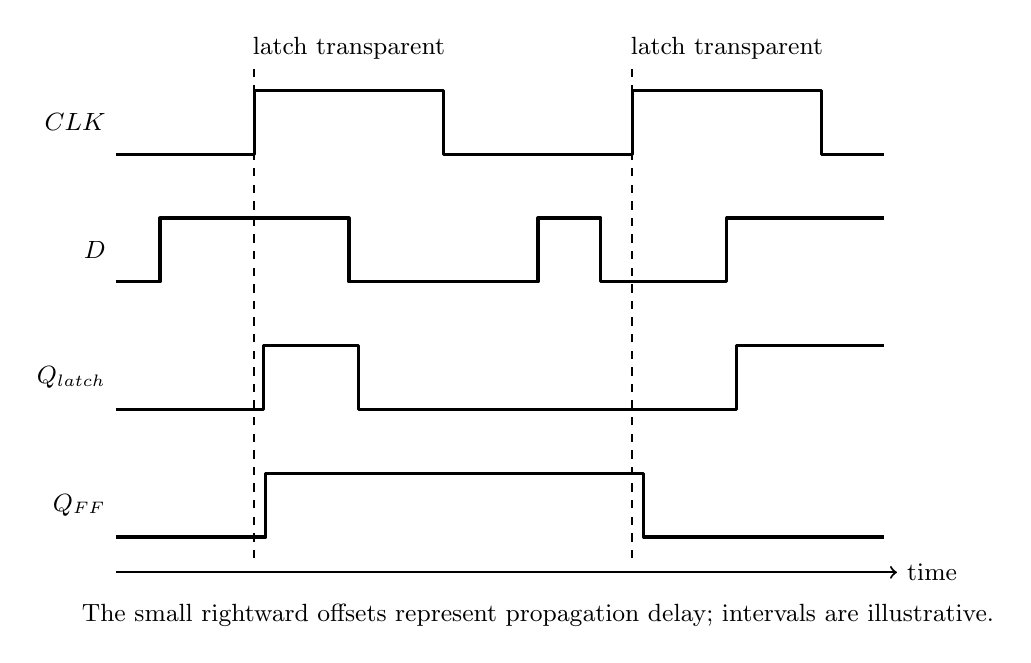
\begin{tikzpicture}[x=0.8cm,y=0.9cm,font=\small,line width=0.75pt,
  thick/.style={line width=1.15pt,line join=round}]
  \draw[->] (0.8,0.25) -- (13.2,0.25) node[right] {time};
  \foreach \y/\name in {6.6/$CLK$,4.8/$D$,3.0/$Q_{latch}$,1.2/$Q_{FF}$}
    \node[left] at (0.8,\y) {\name};

  \draw[thick] (0.8,6.15) -- (3,6.15) -- (3,7.05) -- (6,7.05)
    -- (6,6.15) -- (9,6.15) -- (9,7.05) -- (12,7.05)
    -- (12,6.15) -- (13,6.15);
  \draw[thick] (0.8,4.35) -- (1.5,4.35) -- (1.5,5.25) -- (4.5,5.25)
    -- (4.5,4.35) -- (7.5,4.35) -- (7.5,5.25) -- (8.5,5.25)
    -- (8.5,4.35) -- (10.5,4.35) -- (10.5,5.25) -- (13,5.25);
  \draw[thick] (0.8,2.55) -- (3.15,2.55) -- (3.15,3.45)
    -- (4.65,3.45) -- (4.65,2.55) -- (9.15,2.55)
    -- (10.65,2.55) -- (10.65,3.45) -- (13,3.45);
  \draw[thick] (0.8,0.75) -- (3.18,0.75) -- (3.18,1.65)
    -- (9.18,1.65) -- (9.18,0.75) -- (13,0.75);

  \foreach \x in {3,9}
    \draw[dashed] (\x,0.45) -- (\x,7.35);
  \node[align=center] at (4.5,7.65) {latch transparent};
  \node[align=center] at (10.5,7.65) {latch transparent};
  \node[align=center] at (7.5,-0.35)
    {The small rightward offsets represent propagation delay; intervals are illustrative.};
\end{tikzpicture}
\end{document}
